We use the Sherpa event generator with the standard FastSim sequence
to produce samples of approximately 20,000 \ww\ events with and
without anomalous couplings. We also use MCFM v6.0 NLO generator for
systematic studies and cross-section estimations. The leading lepton
distribution is found to be consistent between the two approaches as
one can see in Figure~\ref{fig:generator_comparison}.
\begin{figure}[tp]
  \centerline{
    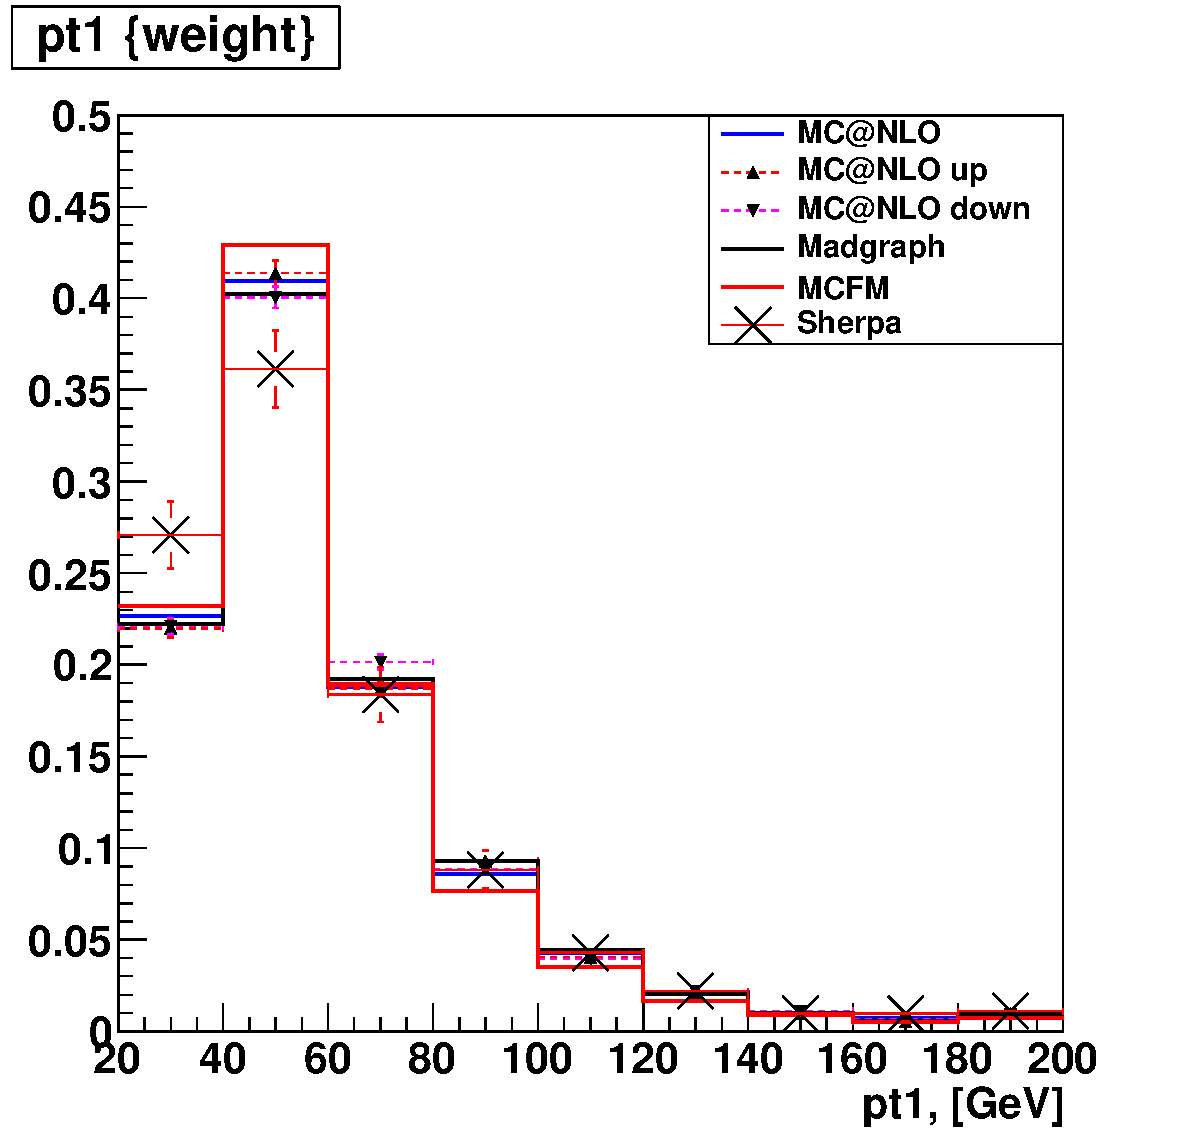
\includegraphics[width=0.45\textwidth]{figures/generator_comparison.pdf}
    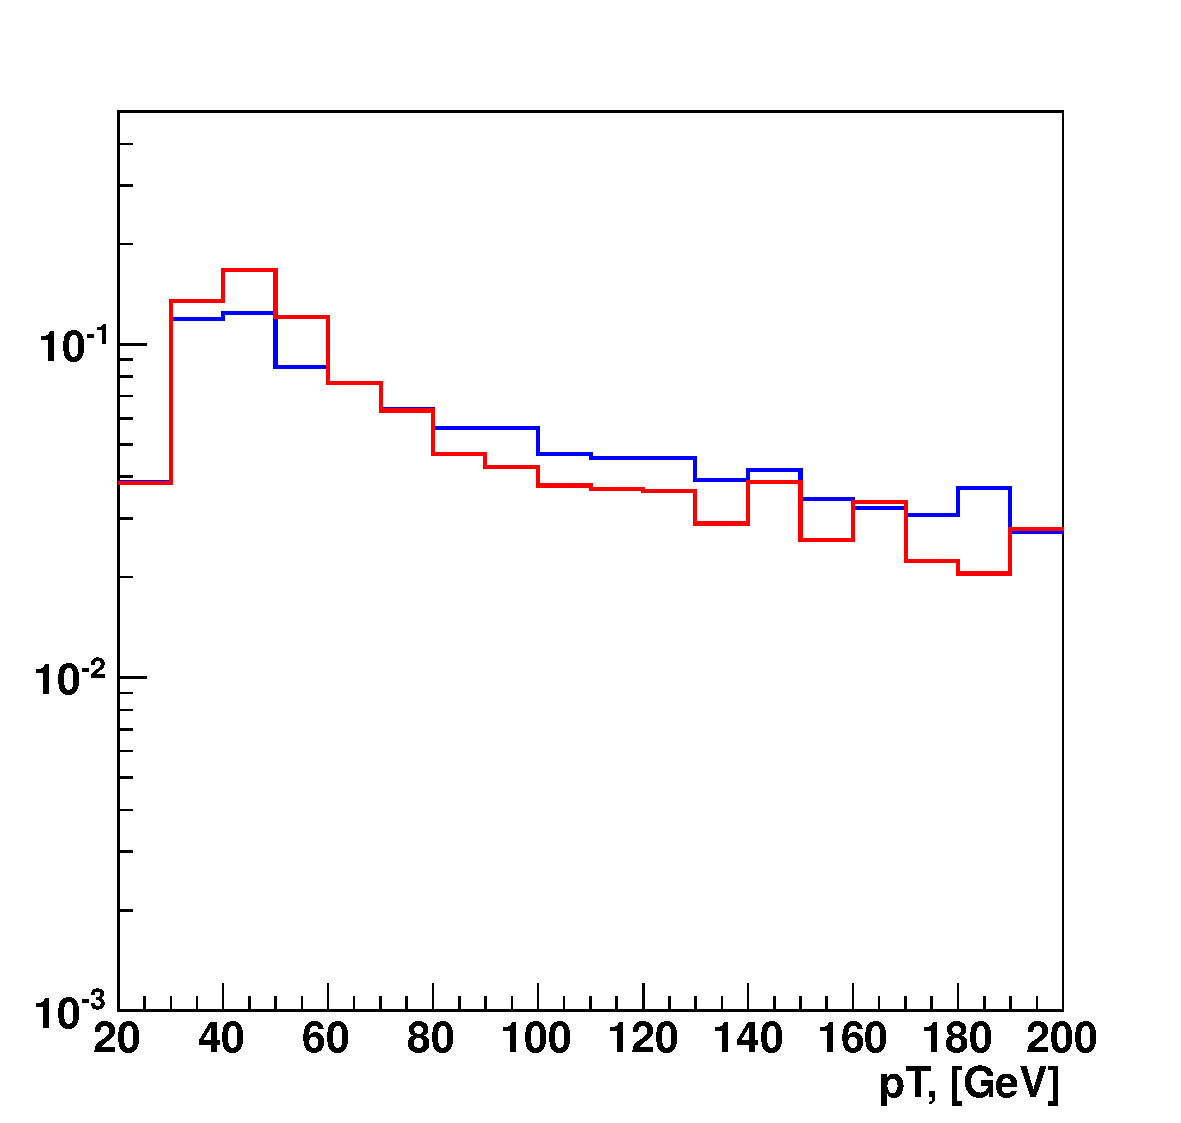
\includegraphics[width=0.45\textwidth]{figures/generator_comparison_atgc.pdf}
  }

  \caption[Generator comparison]{Leading lepton \pt\ distribution
  for \WW\ simulated data using Madgraph+FullSim (black),
  Sherpa+FastSim (blue) and MCFM (red). Left plot shows distributions
  without anomalous couplings. Right plot shows distributions with
  $\lambda_{Z}=0.5$.}

  \label{fig:generator_comparison}
\end{figure}

The anomalous coupling samples were produced with couplings listed in
Table~\ref{tab:xsections} in which one is the Standard Model value,
and the other two coupling values vary.
